\chapter{序論}
\label{chap:introduction}

\section{背景}
\label{sec:background}
近年の少子高齢化に伴い，人の移動や物流の効率化が重視されるようになっている．その需要に応えるため，数人が搭乗する小型モビリティや，歩行者に寄り添って荷物を運ぶモビリティロボットの研究・開発が進められている\cite{honda_ci}．これらのモビリティは，工場や大学の構内，建物に囲まれた区域，屋内外の境界など，高精度地図の整備やGNSSの受信が難しい場所で運用されることが多い．そのため，カメラと車輪速度や慣性計測装置などの内界センサだけで走行できることが求められる．

一方で，このようなモビリティが実用に足る移動時間で運行するためには，安全に走行できる範囲で速度を上げる必要がある．カメラ画像から走行可能な領域や目標経路を推定する手法は数多く提案されているが\cite{bojarski2016,codevilla2018,qin2020}，それらの研究の多くは走行の成功率や経路の推定精度で評価されており，どの速度まで走行できるか，走行時間を決めているのは何かという観点からの評価は少ない．カメラだけで走行する手法は速度を上げると失敗が増えることが報告されているが\cite{drews2017,okelly2020}，その原因が経路の推定，速度の計画，経路の追従のどれにあるのかは切り分けられていない．

\section{AI-Formula}
\label{sec:aiformula}
AI-Formulaは，計測自動制御学会および自動車技術会が主催し，本田技術研究所がサポートする小型モビリティのレース型競技会である\cite{okada2025,okada2024}．競技に用いるモビリティは三輪モビリティであり，本田技術研究所から提供される．Fig.~\ref{fig:mobility}にモビリティを，Fig.~\ref{fig:course}にコースを示す．モビリティは2つの前駆動輪と1つの後従動輪を有し，駆動輪のトルク差で従動輪の向きを変えて旋回する．

2026年度の競技は，指定されたコースを連続して3周する時間を競うタイムアタック形式である\cite{aif_rule2026,aif_rule_mid3}．コースには外周を走行する赤コースと，交差点を通って距離を短縮する青コースがあり，赤コースでは信号に従って停止エリア内に停止し，青コースでは指定された交差点を走行する．コース上にはランダムに配置された静的障害物（コーン）と，外周を低速で周回する動的障害物が置かれ，これらを回避して走行する．ソフトウェアには，LiDARと自作の事前地図の使用禁止，安全機能以外のGNSSの使用禁止という制約が課され，事前地図は運営が提供するトポロジカルマップのみ使用できる．すなわち，カメラと内界センサ，運営提供の粗い地図だけで，信号・交差点・障害物を含むコースを走行しなければならない．これは，\ref{sec:background}節で述べた高精度地図やGNSSに依存しない小型モビリティの運用条件と一致する．

\begin{figure}[H]
  \centering
  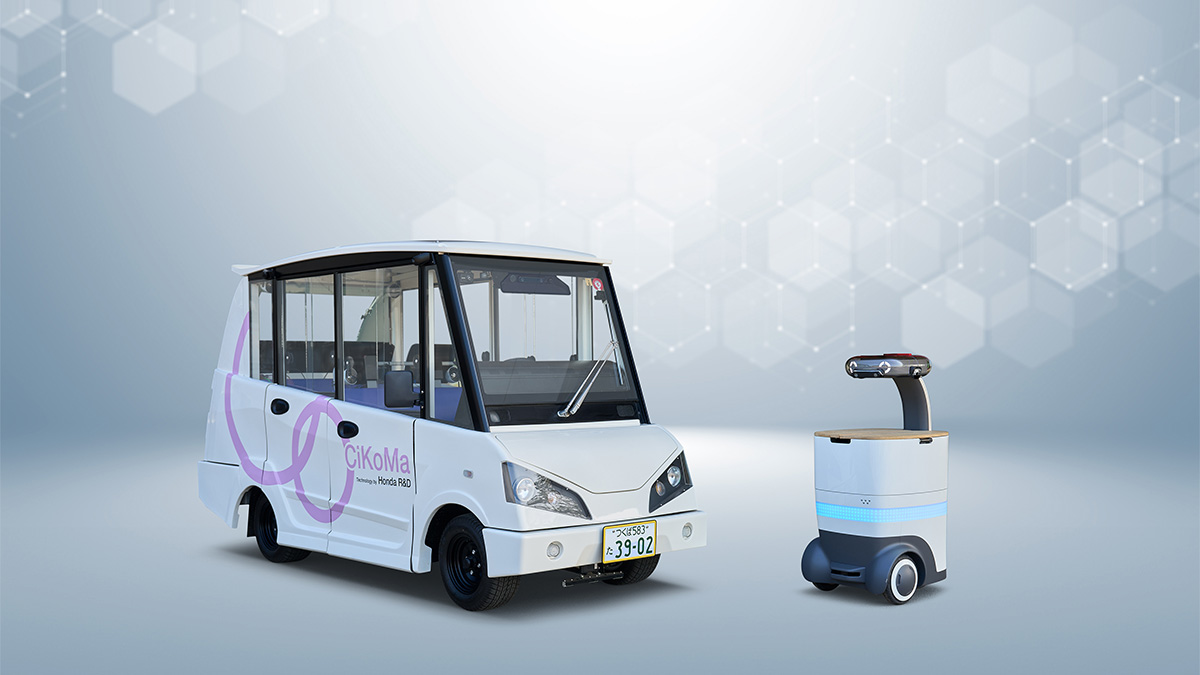
\includegraphics[width=0.7\textwidth]{images/mobility.png}
  \caption{Mobility for AI-Formula. (source: \cite{fujino2026})}
  \label{fig:mobility}
\end{figure}

\begin{figure}[H]
  \centering
  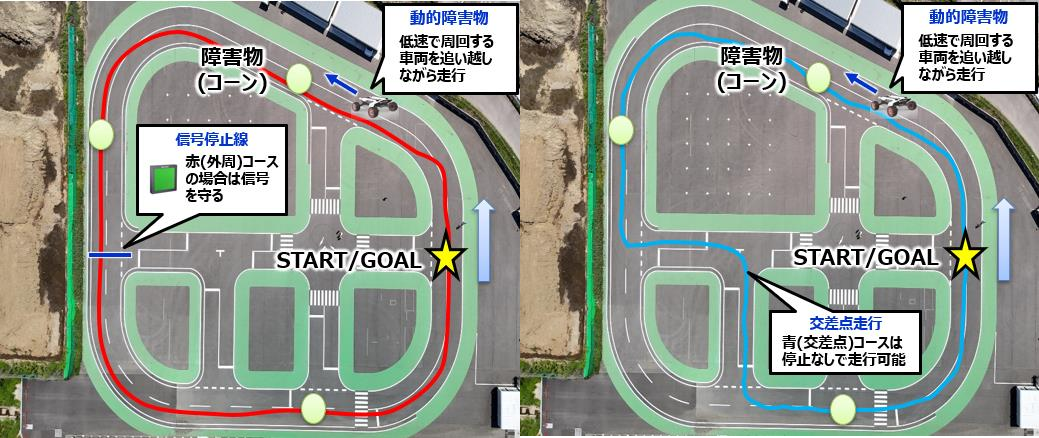
\includegraphics[width=0.95\textwidth]{images/course.png}
  \caption{Course for AI-Formula (left: red course, right: blue course). (source: \cite{aif_rule_mid3})}
  \label{fig:course}
\end{figure}

千葉工業大学チームは2024年度および2025年度の競技に参加しており，2025年度の競技に向けては，従動輪機構と車体制御系の改良\cite{fujino2026}，白線認識を入力とする学習型の経路生成，Frenet座標系に基づく回避経路生成，Pure Pursuit法による経路追従からなる自律走行システムを開発した\cite{yamashita2025si,fujino2025sice}．2026年度の競技に向けては，競技規則の変更に合わせて，カメラ画像から交差点での進行方向に応じた目標経路を生成する経路生成，経路の曲率に基づく速度計画，モデル予測制御による経路追従，信号と障害物に対する停止・回避を新たに開発した．開発したソフトウェアはGitHubで公開している\cite{aiformula_github}．

\section{関連研究}
\label{sec:related}
自律走行車のレースに関する研究は，Betzら\cite{betz2022}が認識，自己位置推定，計画，制御，学習の観点から整理している．Formula Student Driverless向けの全システムを報告したKabzanら\cite{kabzan2020}は，認識から指令までの約300\,msの遅延が最大のボトルネックであり，速度に上限をかけざるを得なかったと述べている．Indy Autonomous Challenge向けのソフトウェアを報告したBetzら\cite{betz2023}は，モジュールごとの計算時間と遅延を実測している．小型車両を用いたF1TENTHでは，条件を揃えて計画方式だけを替えてラップタイムを比較する評価環境が整備されている\cite{okelly2020,evans2024}．これらの研究は，システムの構成と到達したタイムを報告しているが，知覚・計画・制御のどの要素がどれだけ走行時間に寄与したかは定量的に分解していない．また，いずれもLiDARまたはGNSSによる自己位置推定を前提としている．

固定された経路に対する最短時間の速度計画は，加速度の制約を前進・後退計算で満たす方法\cite{lipp2014}や，最小曲率経路と組み合わせる方法\cite{heilmeier2020}として確立している．これらは経路が正確に既知であることを前提としており，カメラで推定した経路のように誤差と時間変動を含む経路に適用したときの走行時間への影響は扱われていない．

カメラ画像から直接操舵を出力するend-to-end学習\cite{bojarski2016}や，交差点での進行方向を条件として与える条件付き模倣学習\cite{codevilla2018}は，走行の成功率で評価されており，速度は評価の対象になっていない．Drewsら\cite{drews2019}は単眼カメラ・IMU・車輪速と概略地図で高速走行を実現しているが，速度を上げたときの失敗の要因は切り分けていない．学習に基づく経路計画の評価については，Daunerら\cite{dauner2023}が，記録データに対するオフライン（開ループ）の指標が実際に走らせた閉ループの性能をほとんど予測しないことを示している．Philionら\cite{philion2020}は，知覚の性能を下流の計画への影響で評価する指標を提案している．これらは，要素の良し悪しを閉ループの走行結果で評価する必要があることを示している．

国内のAI-Formulaに関する発表は，車両側のプラットフォーム\cite{okada2024,okada2025}，カメラによる車線追従\cite{hoshino2025}，各チームの取り組み\cite{fujino2025sice,yamashita2025si}の報告が中心であり，同じ車両・同じコースで方式の違いを走行時間の内訳として比較した例はない．

以上から，カメラと内界センサだけで走行するモビリティについて，経路生成・速度計画・経路追従の各要素が周回時間にどれだけ寄与しているか，また速度を上げたときにどの要素が律速になるかを，実車で定量的に示した研究は見当たらない．

\section{研究目的}
\label{sec:purpose}
本研究では，AI-Formulaに向けて開発した，カメラ画像に基づく経路生成，速度計画，経路追従制御からなる自律走行システムを対象に，各要素が周回時間と完走に寄与した大きさを評価することを目的とする．具体的には，次の3点を明らかにする．
\begin{enumerate}
  \item 実測の周回時間を，車両の限界だけで決まる基準時間と，経路生成・速度計画・経路追従・停止および障害物対応に起因する増加分に分けて示す方法を構成し，実車の走行記録に適用する．
  \item 実車の走行記録から同定した車両応答と経路生成の誤差を組み込んだ閉ループシミュレーションによって，各要素を除いた場合の周回時間と完走の可否を比較し，要素ごとの寄与を求める．
  \item 並進速度の段階ごとに，周回時間や完走を律速している要素がどのように移り変わるかを示す．
\end{enumerate}
本研究では，個々の手法そのものの新規性は主張しない．前進・後退計算による速度計画，Frenet座標系に基づく経路生成，Pure Pursuit法，モデル予測制御，条件付きの学習型経路生成はいずれも既存の手法である．本研究の貢献は，これらを組み合わせた実車システムについて，走行時間を要素別・速度域別に定量化する評価方法と，その適用で得られた知見にある．

\section{研究のアプローチ}
\label{sec:approach}
実車の走行機会は月に1回程度に限られ，同一条件での反復走行を十分に確保することは難しい．そこで本研究では，実車走行をシステムの同定と検証に用い，要素ごとの比較は実車で較正した閉ループシミュレーションで行う．閉ループシミュレーションには実際に車両で動作しているソフトウェアをそのまま用い，車両の応答と経路生成の誤差は実車の走行記録から同定したモデルで置き換える．シミュレーションが実車の走行記録を再現することを確かめたうえで，要素を1つずつ除いた条件の周回時間と完走の可否を比較する．実車では，並進速度の段階ごとに数本の周回走行を行い，周回時間の内訳とシミュレーションの予測を照合する．

この方法は，類似するモビリティの開発において，限られた実車機会で改良の効果を見積もるための手順としても用いられることを意図している．

\section{論文の構成}
\label{sec:organization}
本論文は以下の構成で記述する．1章では本研究の背景と目的について述べた．2章では，対象とするモビリティと，本年度開発した自律走行システムの構成を昨年度との差分とともに述べる．3章では，周回時間を要素別の増加分に分解する方法と，閉ループシミュレーションの構成を述べる．4章では，実車走行の結果と周回時間の内訳，速度を上げたときの失敗の要因を述べる．5章では，閉ループシミュレーションによる要素ごとの寄与の比較と，速度段階ごとの律速要因について述べる．最後に，6章では本研究のまとめと今後の展望について述べる．
